\section{Design} % (fold)
\label{sec:design}
The main goal of the Realms system is to help in the creation of simple location-based applications using a configuration process. The system consists of the following two major components:
\begin{itemize}
	\item The \emph{configuration manager} - empowers users with the possibility of augmenting a physical space with virtual properties and rules (we call it a Realm). It also has the responsibility of storing the configured Realms and provide an API\footnote{Application Programming Interface} for the mobile clients
	\item The \emph{mobile client} - collects relevant context data and intermediates the interaction between the users and the system
\end{itemize}

\noindent In the beginning we had designed for a generic system taking into account a large variety of possibilities. In order to create an actually working prototype, we had to reduce the complexity, meaning that we have designed a system with a limited set of features. To be more specific, the configurator allows users to manage their realms (create, delete and edit). A realm is made up by a set of \emph{Markers}\footnote{a virtual property characterized by a (latitude, longitude, radius) tuple, augmenting a physical location with virtual data} that can be either a \emph{Question} or an \emph{Information}. Semantically this means that the user configuring the Realm can augment a location either with information that could be useful to the Realm user (e.g. historical data about an old building)  or a question that a user of the Realm can answer. Given the three characteristics of a marker (latitude, longitude, radius) we can say that it augments an area rather than a single point. This is necessary because positioning with "0" accuracy is hardly achievable with today's positioning technologies. Furthermore, augmenting an area with a variable radius (of the Realm configurator's choice) provides a more flexible configurator (even with the possibility of augmenting an area with radius "0", that is a single point).
\\

\noindent From a hardware perspective, the mobile client is meant to run on a mobile platform (i.e. such as Android, iOS etc.) enabled with the necessary technologies to collect location data (i.e. GPS, mobile network, wi-fi). Although most mobile devices running one of the required platforms support internet connection, we would like to note that this is a mandatory requirement. The realms server is intended to run on a stationary computer connected to the internet.
\\

\noindent There are two end user types which will use our system: the realm managers, which create realms using the Realm configurator, and the realm users which interact with the realms using the provided mobile client. Actually, the mobile client users are end-users both to us and the Realm managers: they are our end-users because they use the mobile client, that we provide, to connect to one of the Realms, provided by realm managers. To make a clear distinction between the components each user type interacts with, we have illustrated a system usecase scenario in Figure \ref{fig.system_usecase}. From the usecase we can conclude that the realm managers connect through a web-based interface to the reams server which enables them to manage their realms, while the realm users connect to the realms server using the provided mobile application.
\begin{figure}
	\centering
	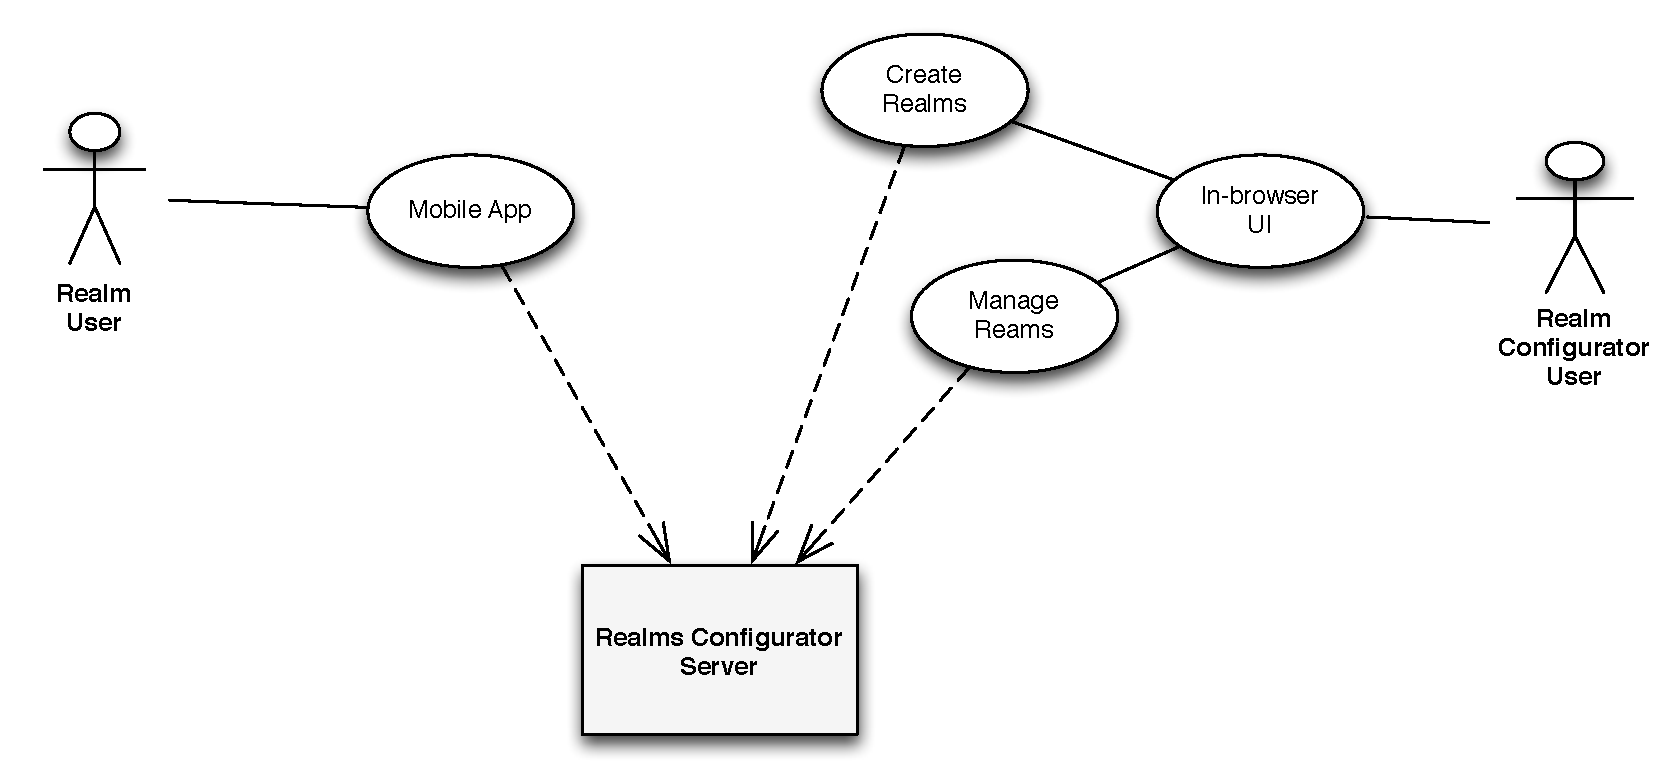
\includegraphics[width=1.0\linewidth]{fig/system_use_usecase}
	\caption{Realms system usecase scenario}
	\label{fig.system_usecase}
\end{figure}
\\

\noindent Indoor positioning needs a lot more infrastructure than the one provided by GPS satellites which makes indoor locations hard to deal with. Hence, we consider indoor spaces to be out of scope for our system and the realms which a configuration manager will be able to create can be based only on outdoors spaces.
\\

\noindent The main advantage over similar systems is that we empower users to create a ready-to-be-used location-based application without writing one line of code.
\\

\noindent The system is made up by a mobile client and a central infrastructure, thus the nature of the system is distributed. The natural choice to design such a system is to follow the client-server model \cite{Coulouris:2005}.
\\

\begin{figure}
	\centering
	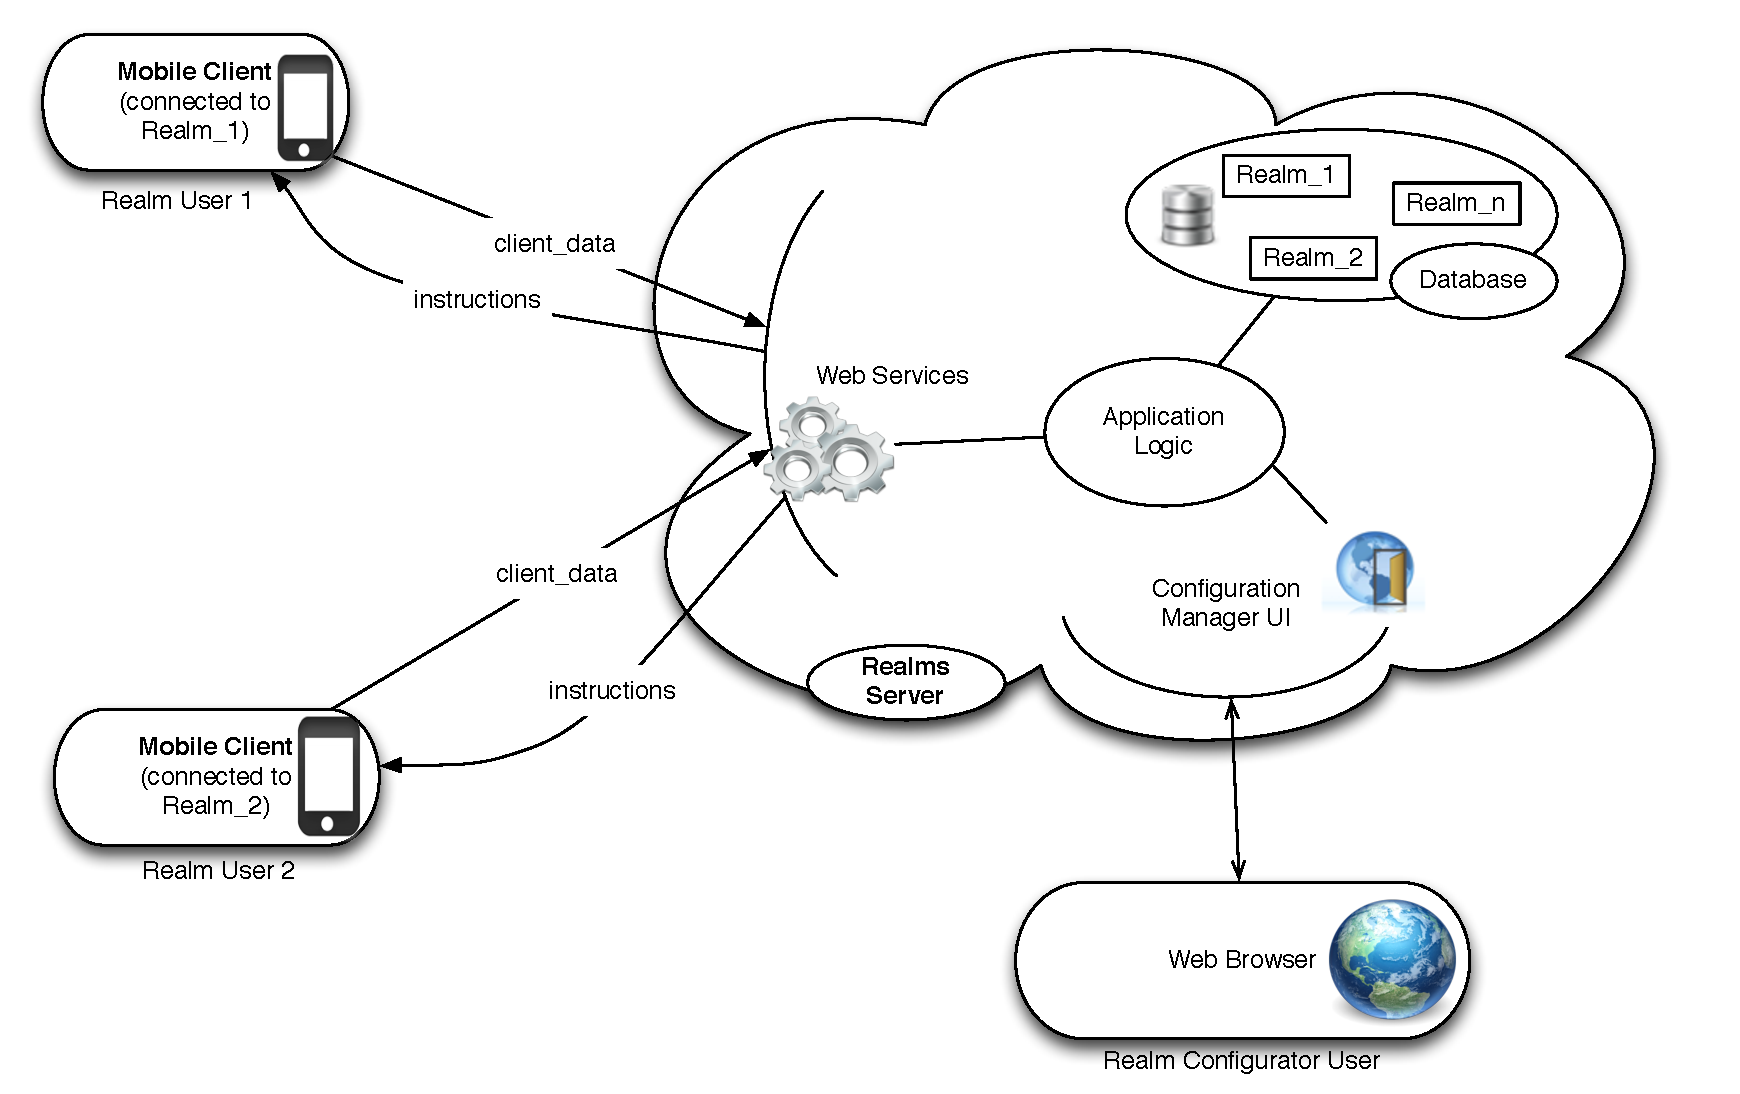
\includegraphics[width=1.0\linewidth]{fig/realms_high_lvl}
	\caption{High level system overview}
	\label{fig.design.high_lvl}
\end{figure}
\noindent Figure \ref{fig.design.high_lvl} depicts the major components and data structures of the system. The configuration manager is a standalone web application running on a stationary computer (the realms server) and is made up by the following subcomponents:
\begin{itemize}
	\item a database assuring the persistence of configured realms
	\item the application logic that holds the processing routines which take place behind the scene
	\item two interfaces to be accessed from the outside by the different clients of the system - a set of web services to be accessed by the mobile clients and a configuration UI (user interface) to be accessed by the realm configurators through a web browser. 
\end{itemize}

\noindent Before we go any further, we would like to shortly address the concrete choices we have made in the design based on the 4 dimensions identified in Section \ref{sub:taxanomy_of_location_features}:
\begin{enumerate}
	\item The location is represented in absolute values expressed in terms of latitude, longitude and radius which represents raw location data. In the future, this can easily be expressed as symbolic or relative applying if needed, by simply applying a few transformations on top of the raw data.
	\item For the location level have employed both levels. Location-based interactions happen when realm users receive information from the realm server based on their actual location. The realm user might be prompted to provide feedback in certain situations and the outcome of the interaction is the feedback of the user which is recorded in on the server side - this is characterised as a location-enhanced interaction.
	\item As data types, both information and commands are present. Information is the data type generated when realm users receive information based on their actual location, while providing feedback based on the current location (and associated data) is done thought a location-based command.
	\item The communication type we have employed is based exclusively on request-based. That is, the user has to explicitly query the server for updates (i.e. by pressing a button).
\end{enumerate}
\\

\noindent Finally, we will shortly address the architecture we base our API for the mobile clients upon. As discussed by Fielding in \cite{Fielding:2000}, REST is an architecture style for distributed hypermedia systems. A web service is an API which is accessed through the HyperText Transfer Protocol (HTTP) and executed on a remote system, hosting the requested service. A RESTful web service is a web service implemented using HTTP and the principles of REST. The RESTful web service is defined by a collection of resource, each of which is defined by three main characteristics:
\begin{itemize}
  \item the base URI identifying the web service
  \item the MIME\footnote{Multipurpose Internet Mail Extensions} type of the
  data supported by the web service (JSON, XML, etc.)
  \item the web service's interface defined against the HTTP supported methods
  like POST, GET, PUT, DELETE etc.
\end{itemize}
The REST architectural style imposes a client-server architecture, which fits well our system's architecture, which is also based on a client-server approach.

\subsection{Configuration Manager} % (fold)
\label{sub:configuration_manager}
\noindent The role of the configuration manager is on one hand, to present a realm configurator users with an interface where physical spaces can be configured with markers, on the other hand to provide an API for the mobile clients and handle their requests.
\\
The most intuitive interface to augment physical location is probably a virtual map which can be easily be browsed for concrete physical locations (latitude and longitude), city name, place name, address etc. These features make it easy for the user to rapidly find the desired location they want to augment. The configuration process results in a list of configured realms, each realm holding a set of Markers. As the system is centered around the data, we have created a concrete design for the database to start with. The  "realms" database diagram, illustrated in Figure \ref{fig.db_structure}, depicts in details the data structure of the system. Each realm configurator user is characterised by the "user" data structure. Besides attributes like username and password a user has attached a list of realms he has created. A "realm" augments a physical area based on the (latitude, longitude, radius) tuple and is characterised by a name and a description. As realms are now positioned at concrete coordinates, mobile clients will be able to see, and therefore communicate, only with realms in their coverage/vicinity.
\begin{figure}[H]
	\centering
	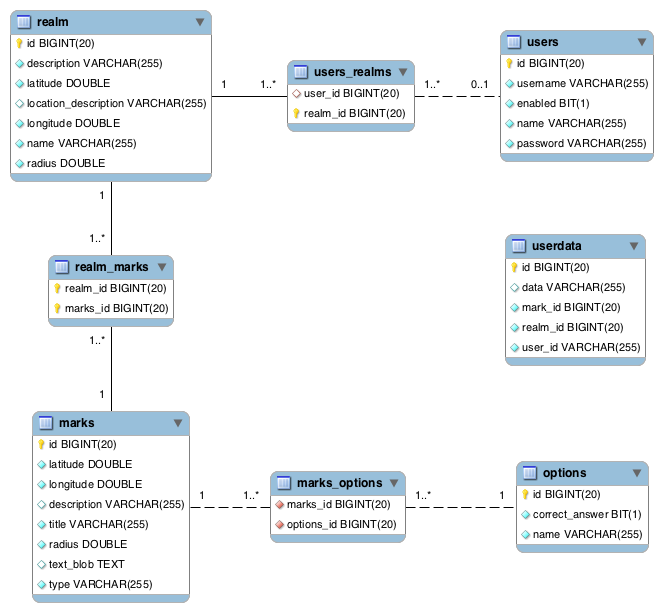
\includegraphics[width=1.0\linewidth]{fig/db_structure}
	\caption{Realms database diagram}
	\label{fig.db_structure}
\end{figure}
\noindent A realm contains a set of "markers" positioned within the realm (they are not relative to the realm, but absolute in the same coordinate system as the realm is). Markers also augment physical areas based on the (latitude, longitude, radius) tuple and are characterised by title, type\footnote{for now we only have information and question as marker type} and text blob. The text blob is interpreted based on the marker type: for an information it simply represents information about the augmented location, whereas for a question it represents a question the mobile client will be asked. A Marker might have a list of "options" which represent possible ratings a user can use to rate an information marker or possible answers for a question marker. The "userdata" data structure is used to record the user feedback from mobile clients, which can later be presented in the UI from the realm configurator users.
\\

\noindent Based on the above described data structures, we have designed a RESTful API to be used by the mobile clients. We have decided not to use any authentication for the current protocol as it would have introduced extra complexity as security is not the main concern in this current state. Although we have taken a trivial security method: each service requires the userID as a parameter and if the user's ID is not present, the service will not fail taking any action. For each service we will specify, in brackets, the concrete values we have used for each of the design dimensions identified in Section \ref{sub:taxanomy_of_location_features}. The API provides following services:
\begin{itemize}
	\item \emph{getRealms(lat, lon, userid)} -- return all the realms the given coordinates are positioned in [absolute location representation, location-based interaction, information data type, request-based communication]
	\item \emph{getMark(lat, lon, realm, userid)} -- return one mark covering the given coordinates from the specified realm [absolute location representation, location-based interaction, information data type, request-based communication]
	\item \emph{rateInfo(reakmid, markid, rating, userid)} -- provide feedback for an information marker type by rating it [absolute location representation, location-enhanced interaction, command data type, request-based communication]
	\item \emph{markOption(reakmid, markid, optionid, userid)} -- provide feedback for a question marker type by answering the question choosing one of the provided answers [absolute location representation, location-enhanced interaction, command data type, request-based communication]
\end{itemize}
\\

\noindent To characterise the API in a few words, we have designed a client-server interaction based on the request-reply programming model \cite{Coulouris:2005}.
% subsection configuration_manager (end)be available having 

\subsection{Realms Android App} % (fold)
\label{sub:realms_android_app}
The mobile application presents users with the ability to access realms and find markers based and provide feedback for them. Figure \ref{fig.design.mobile_client} depicts the main data structures and the interface the mobile client should implement to communicate with the realms server.
\begin{figure}[H]
	\centering
	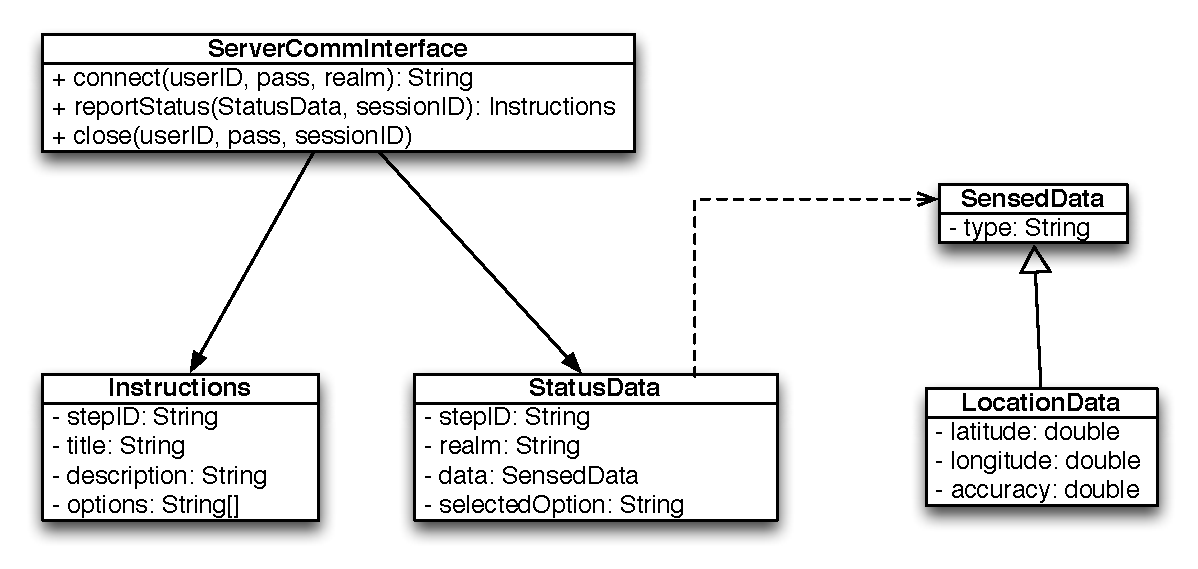
\includegraphics[width=1.0\linewidth]{fig/mobile_client}
	\caption{Data structures and communication interface which allows the mobile client to communicate with the realms server}
	\label{fig.design.mobile_client}
\end{figure}
\begin{figure}[H]
	\centering
	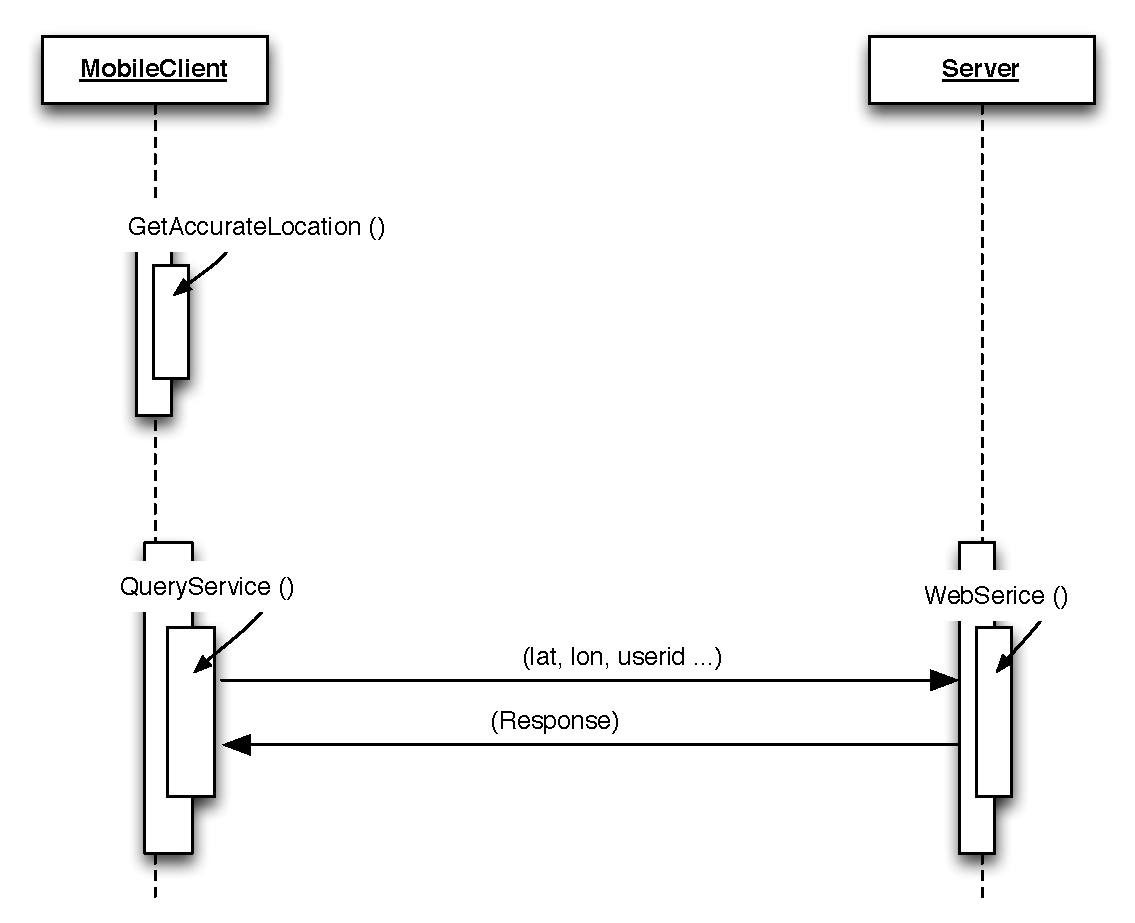
\includegraphics[width=1.0\linewidth]{fig/abstract_communication_protocol}
	\caption{Communication Protocol}
	\label{fig.design.comm_protocol}
\end{figure}
\noindent Figure \ref{fig.design.comm_protocol} further details the interaction between the mobile client and the server. Before any communication can take place, we need to assure that the client has the latest location conforming to a good-enough accuracy. Once accurate location data is available, the client can perform a location-enhanced or location-based interaction.
% subsection realms_android_app (end)
% section design (end)